\graphicspath{ {../body/bayesian_figures/}}
\chapter{基于Bayesian博弈模型的资源分配算法}
%\label{chap_bayesian_game}
\par 
本章研究的目的是,在尽可能少的收集用户信息的情况下,
不通过集中决策,而让用户自身来决策与协商分配系统的资源。
我们首先提出一个新的业务类型描述方式。
与以往的离散业务类型描述方法不同,我们将用户的业务类型描述成一个连续的随机变量。
然后建立了一个基于Bayesian博弈的竞争与决策模型。
这个模型可以有效地描述在不完备信息下的用户资源竞争的情况。
通过建立适当的收益与惩罚机制,激励用户根据自身的业务情况做出理性的分析和决策;既可以保证自身的服务质量,
又能让资源得到充分利用,避免贪婪用户过多地占用宝贵的系统资源。
%
\section{引言}
由于无线资源稀缺,研究者在无线资源分配及管理方面做了许多意义的工作。
近年来,博弈论做为经济学家常用的数学方法也被引入到无线网络技术研究领域,
特别是针对Ad Hoc网络或无线传感器网络\cite{Srivastava:2005}\cite{FangBensaou2004}。
博弈论的本质是通过数学模型来研究多个利益冲突的理性个体如何调整自己行为的理论。
通过构造合适博弈论模型及其博弈规则,可以引导自私但又理性的个体做出既有利于自已又利于其他参与者的决策。
例如,在多媒体码率分配问题中,用户往往为了保证自身最佳的服务质量,会过多地占用系统的资源,
进而导致整个系统性能的下降。
为此,学者Zhang和Liu针对这个问题,提出竞价博弈及相应的税制机制来限制用户这种过分贪婪的行为\cite{ZhangLiu2011}。

但是,这些方法都通常会有一个比较严格的假设:
在这类博弈中,每个博弈参与者或用户都要具有其他参与者或用户的完备信息。
并且,在博弈过程中,设置一个集中控制的单元负责传递用户之间的各种信息。
例如,在文献\cite{ZhangLiu2011}中,用户的各种私有信息,收益函数的参数等等都要在用户之间进行交换。
这样会导致大量的信息在用户之间传送。
这类博弈分析模型称之为完备信息下博弈模型。
通常,在博弈论研究中,所有参与者知识完备的假设是一个简单而又恰当的近似。
在有些实际的问题中,这种假设过于理想和完美。
例如,根据用户业务类型来进行网络资源分配的问题。
因为随着移动互联网的发展,用户业务种类越来越多,越来越细致。
所以,想在资源分配之前,通过集中控制单元准确获取所有用户对资源的精确需求比较困难。
博弈论中有这样一种类型的博弈:一些参与者可能不知道其他参与者的收益。
这种类型的博弈被称之为“不完全信息的博弈”,或者被称为“Bayesian博弈”。

在本章中我们利用这种新的分析模型:Bayesian博弈分析模型,对系统中参与者的行为进行引导。
这种分析模型与完备信息博弈模型不同。
每个用户除了对自身的情况一清二楚之外,对参加博弈的其他用户的信息并不十分了解。
也就是说他所得到的其他用户信息是不完整的;或是说,每个用户的私有信息是受到一定程度的保护。

\section{业务类型与系统博弈模型}
\subsection{离散与连续的业务类型}
目前,绝大多数的文献对于用户业务的类型讨论都是基于离散的分类形式。
例如,在早期的无线GSM网络中,话音几乎是唯一的业务。
随着网络技术的发展,除了话音外,文字、图片和视频等数据业务相继出现。
不同阶段的通信标准也根据其特点,规定了业务的种类。
比如,3GPP定义了四种基本业务类型,即会话类业务、流媒体业务、交互类业务和背景类业务。
IEEE802.16e中定义了这五种业务类型:UGS,rtPS,ertPS,nrtPS,BE。
在分类的原则上,有的的分类是指从应用层的角度来看待网络承载的数据,例如视频或声音。
有的分类是从网络传输的角度来看。不同的业务类型代表了不同业务对网络性能的要求,如对带宽、时延等等。
假设业务分类可以从概论论的角度来看,那么用户所承载的业务类型的一切可能的结果(离散的)也就可以组成的集合是一个样本空间~$\Omega$~,
那么空间中元素就可以对应为目前网络传输中的一种业务类型定义。

然而,我们如果仔细思考就会发现,这种离散的业务分类方法是有很大的局限性:过于庞统。
譬如,对于同一个视频片段,不同的编码器(MPEG4,H.264,H.265)或同一种编码器的不同编码设置参数都会对视频流的结果产生影响。
对于物理层调制编码,不同的信道模型和编码方法也同样会对数据产生影响。

所以,我们认为除了原有的离散式的业务类型定义以外,还可以将这种离散式分类方法推广到连续式的业务分类方法。
这可能更接近业务本来的面目。
在连续的情况下,业务类型其实是一个概率意义上的随机变量~$X$~,并且服从某个概率分布~$F(x)$~。
每一种现实存在的业务类型都是这个随机的变量的一个取值。下面我们将这种业务分类连续定义思想应用到Bayesian博弈模型中。

\subsection{博弈模型}
假设在一个无线网络基站的覆盖范围内,目前有~$N$~个在线用户正在共享无线资源进行通信。
为了能够更加公平且有效的使用资源,基站控制器会在有新的用户进入的时候,
触发一次资源调整的方案。调整的目的是让用户根据目前自身的业务情况,重新申请合适的资源数量,
避免一些用户长期大量占用资源。
例如,在IEEE802.16标准中,
基站控制器可以通过引导各个用户投票来竞争所需要的资源。
但是由于资源有限,随着用户的数目逐渐增多,竞争就会加剧。
有时会出现先接受服务的用户为了保证自身的服务质量,申请多于自身需求资源且不加以释放。
如果对这种贪婪用户的情况不能有效地加以处理,那么结果会让整个系统的资源利用率恶化。
为了能从机制上规范所有用户的资源使用行为,改变其自身的资源多占用策略。
我们希望通过Bayesian博弈的方式,引导用户根据自身真实的需求进行理性的资源申请和使用。

在我们的博弈模型中,有~$N$~个博弈的参与者(Players)。
每个参与者都要在这个博弈过程中做出这样的决策:是否同意根据目前自身的情况,改变自己资源占用数量。
相应的,参与者有两种选择:“同意”或是“拒绝”。
这种选择形式是典型的~$0-1$~决策。
在决策之前,每个用户都要理性且独立地评估自己的成本~$c$~。
为了鼓励“同意”行为,在博弈机制设计中设置奖惩办法。
如果他选择“同意”,我们提供奖励收益~$b$~。
如果参与者选择“拒绝”,那么参与者的奖励收益~$b$~为~$0$~。
同时,对选择“拒绝”的参与者设置了有条件的惩罚系数~$\tau$~:
如果至少有一个其它的参与者选择“同意”,那么这个选择“拒绝”的参与者才会被惩罚。
也就是说,当在线的所有参与者都决策“拒绝”,
那么意味着当前网络资源利用率已经达到了饱和的上限。
因此,所有选择“拒绝”参与者不会受到惩罚。

对于我们博弈模型,我们做如下的假设:
\begin{itemize}
    \item 假设参与者的奖励收益与惩罚是公共知识。这个信息被所有博弈参与者提前广播通知到的。
    \item 假设参与者的成本是一个随机的变量,服从某个概率分布。同时,只有参与者本身知道自己成本具体的数值。
    因为参与者的业务类型不同,所以我们使用参与者成本表征参与者的业务类型特征。
    \item 假设对于每个参与者自身的成本,我们认为是私有的知识,其他的参与者并不知道。
    这里需要注意是,参与者虽然不知道其他参与者成本随机变量的具体数值,但是知道这个随机变量的分布函数。
    之所以做这样假设的原因是,在实际中我们可以通过统计的方法获得参与者类型的概率分布。这个信息也是公共知识。
    \item 假设所有参与者成本随机变量是独立同分布的,并且其累积概率分布函数~$P(\cdot)$~在区间~$[C_{\min}, C_{\max}]$~是连续增函数,
\end{itemize}
%其中~$0 \leq C_{\min} < C_{\max}$~,且我们设 ~$P(C_{\min})=0$~,~$P(C_{\max})=1$~。

首先,我们定义博弈的策略。
对于任意一个参与者而言,他的策略选择可以用变量~$s_i$~来描述,如\eqref{eqn:chap_bayesian_strategy_definition}所示。
\begin{align}
    s_i = \begin{cases}
        0, \qquad\text{拒绝}\\
        1, \qquad\text{同意}\\
    \end{cases}
    \label{eqn:chap_bayesian_strategy_definition}
\end{align}
其中,此函数的定义域是成本区间~$[C_{\min}, C_{\max}]$~,值域是集合~$\{0,1\}$~中取任意一个值。
“~$1$~”表示参与者愿意“同意”;“~$0$~”表示参与者“拒绝”;
~$i$~表示参与者的序号索引。

然后,我们定义博弈中具有奖惩机制的参与者收益。

对于参与者~$i$~来说,他的收益函数定义为:
\begin{equation}
 u_i(s_i, s_{-i}, c_i, b, \tau) = s_i\cdot (b - c_i) - \max\{s_{-i}\} \tau
\label{eqn:chap_bayesian_player_payoff}     
\end{equation}
其中,记号~$-i$~表示除参与者~$i$~之外的其它所有参与者。
记号~$s_{-i}$~表示其他参与者~$-i$~的策略选择集合。
~$c_i$~表示参与者~$i$~的成本。
~$\max\{s_{-i}\}$~表示在其它所有参与者的策略中选择最大的值。
%
\section{Bayesian博弈分析}
对于每一个理性且自私的博弈参与者,他总想通过自己的选择来使自己的收益最大化。
如果写成纯策略的形式为~$\max(u_i)$~。
策略形式的优点在于每个用户的选择具体直观,
对于所有参与者的选择来说,Bayesian均衡可以用一个策略向量~$( s_1^*(c_1^*),\ldots, s_N^*(c_N^*) )$~来描述。
其中,策略~$s_i^*(c_i^*)$~使得~$E(u_i)$~达到最大值。

但是,求解纯策略问题本质是一个$N$目标优化的极其复杂问题,这是我们所不希望看到的。
所以,为了避免问题的复杂化,我们求解混合策略。
混合策略是纯策略上的一种概率分布。每个博弈参与者的随机化及其他参与者的随机化是统计独立的。
如果使用混合策略,那么问题会转化为最大化参与者的期望收益,~$\max{E(u_i)}$~。
相应的Bayesian博弈的解就是博弈参与者选择“同意”或“拒绝”的概率。

下面我们来具体分析这个博弈。
首先我们引入一个均衡概率的定义~$\theta_{-i}$~。
它表示对于参与者~$i$~而言,至少有一个其他的参与者的决定是“同意”的概率。
通过这个概率定义的引入,我们使得博弈参与者~$i$~与其它博弈参与者的决策行为相关联。
并通过这个定义来表征参与者之间的博弈行为。
这个概率的具体表达式如\eqref{eqn:chap_bayesian:at_least_one_probability}所示。
\begin{equation}
    \theta_{-i} = \hbox{Prob} \Bigl\{ \max\{ s_{-i}\} = 1 \Bigr\} 
    \label{eqn:chap_bayesian:at_least_one_probability} 
\end{equation}
所以,对于一个给定的博弈参与者~$i$~,他的期望收益可以定义为如下公式:
\begin{align}
     E(u_i) &= \theta_{-i} [s_i(b-c_i) -\tau] + (1-\theta_{-i}) (s_i(b-c_i) - 0) \notag\\ 
     &= s_i(b-c_i) - \theta_{-i}\tau
    \label{eqn:player_expe_payoff}
\end{align}

从\eqref{eqn:player_expe_payoff}可以看出,为了使得~$E(u_i)$~尽可能大,在考虑决策的前提下,可以分成两种情况。
如果博弈参与者~$i$~的成本~$c_i$~小于~$b-\theta_{-i}\tau$~,那么参与者~$i$~的决策就是“同意”,也就是~$s_{i}=1$~。
如果~$c_i > b - \theta_{-i} \tau$~,那么参与者~$i$~会选择“拒绝”,~$s_i = 0$~。
那么我们可以将其写为一个分段函数的形式。
\begin{align}
    s_i(c_i) = \begin{cases} 1, &\text{if $c_i < b -\theta_{-i}\tau$;}\\
        0, &\text{if $c_i > b -\theta_{-i}\tau$.}\\ \end{cases} 
    \label{eqn_equilibrium_strategy} 
\end{align}
从\eqref{eqn_equilibrium_strategy}可以看出,参与者~$i$~的成本对决策的影响很关键。
如果他的成本~$c_i$~在区间~$ [C_{\min}, c_i^*] $~,参与者的决策就是“同意”。
其中,我们把~$c_i^*$~称为均衡临界成本。
所以,我们需要求得参与者~$i$~选择“同意”概率,也就是均衡临界成本的概率~$P(c_i^*)$~。
\begin{align}
    P(c_i^*) = \hbox{Prob} \Bigl\{ C_{\min} < c_i \leq c_i^* \Bigr\} 
    \label{eqn:chap_bayesian:equil_prob_c_i}
\end{align}
而且,
如果存在这样一个均衡临界成本,
并将\eqref{eqn:chap_bayesian:equil_prob_c_i} 代入\eqref{eqn:chap_bayesian:at_least_one_probability},
那么就有:
\begin{align*} 
    \theta_{-i} &= \hbox{Prob} \Bigl\{ \max\{ s_{-i}^*\} = 1 \Bigr\} \\ 
    &= 1- (1-P(c_1^*))(1-P(c_2^*))\cdots(1-P(c_{i-1}^*)) (1-P(c_{i+1}^*)) \cdots(1-P(c_N^*)) \\ 
    &= 1- \prod_{j\in\{-i\}} [1-P(c_j^*)] 
\end{align*}
同时,从\eqref{eqn:chap_bayesian:at_least_one_probability}和\eqref{eqn_equilibrium_strategy}可知,
均衡临界成本 ~$c_i^*$~是用户决策的关键值。它关系到用户选择的转换。
因此,均衡临界成本还要满足下面\eqref{eqn_equilibrium_cost}
\begin{align}
    c_i^* &= b - \theta_{-i} \tau \notag\\
    &= b - \tau + \Bigl[ \prod_{j \in\{-i\} } [1 - P(c_j^*) ] \Bigr] \tau
    \label{eqn_equilibrium_cost} 
\end{align}
又因为,对于博弈中的任意一个~$c_i, i=1,\ldots, N$~,都要满足\eqref{eqn_equilibrium_cost}。
假设所有参与者的成本随机变量是独立同分布的,因此~$c_i, i=1,\ldots, N$~之间是可以互换的。
如果存在一个唯一的~$c^*$~,且满足任一个\eqref{eqn_equilibrium_cost},
那么它们值相等,且可用\eqref{eqn:chap_bayesian:equilibrium_cost_equation}来计算得出。
\begin{align}  
    c_i^* &= c^* = b - \theta_{-i} \tau \notag\\ 
    &= b - \tau  + \Bigl[ \prod_{j \in\{-i\} } [1 - P(c_j^*) ] \Bigr] \tau \notag\\ 
    &= b - \tau + \Bigl[ [1 - P(c^*)]^{N-1} \Bigr] \tau
\label{eqn:chap_bayesian:equilibrium_cost_equation}
\end{align}

因此,对于我们提出的Bayesian博弈模型而言,网络中博弈参与者成本(用户业务类型)的概率分布情况会对博弈结果起着关键的影响作用。
%%%%%%%%%%%%%%
\section{不同成本概率分布的分析与讨论}
下面,我们假设博弈参与者成本(业务类型)为两种最常见的概率分布形式,并分别对其进行分析与讨论。
\subsection{均匀分布的情况}
均匀分布是连续概率分布函数中最常见和最简单的。它在所有的概率分布中占着重要的地位。
许多实际上重要的随机变量者服从或是近似服从均匀分布。
此处,我们假设参与者的类型的概率分布~$P(\cdot)$~是在区间~$[C_{\min}=0, C_{\max}=1]$~上的均匀分布。
它的概率密度函数为
\begin{align}
    f_(c) = \begin{cases} c, &\text{if ~$c \in [C_{\min}=0, C_{\max}=1]$~;}\\
        0, &\text{others}\\ 
    \end{cases} 
    \label{eqn_equilibrium_prob} 
\end{align}
其中,我们假设对于参与者的成本被认为是归一化的。
概率密度函数与分布函数图形如\figref{fig:chap_bayesian:uniform_density_scheme}和\figref{fig:chap_bayesian:uniform_cdf_schem}所示。
%%%%%%%%%%%%%%%%%%%%%%%%%%%%%%%%%%%%%%%%%%%%%%%%%%%%%%%%%%%%%%%%%%%%%
\begin{figure}[tb] 
  \begin{minipage}[t]{0.5\linewidth} 
    \centering 
    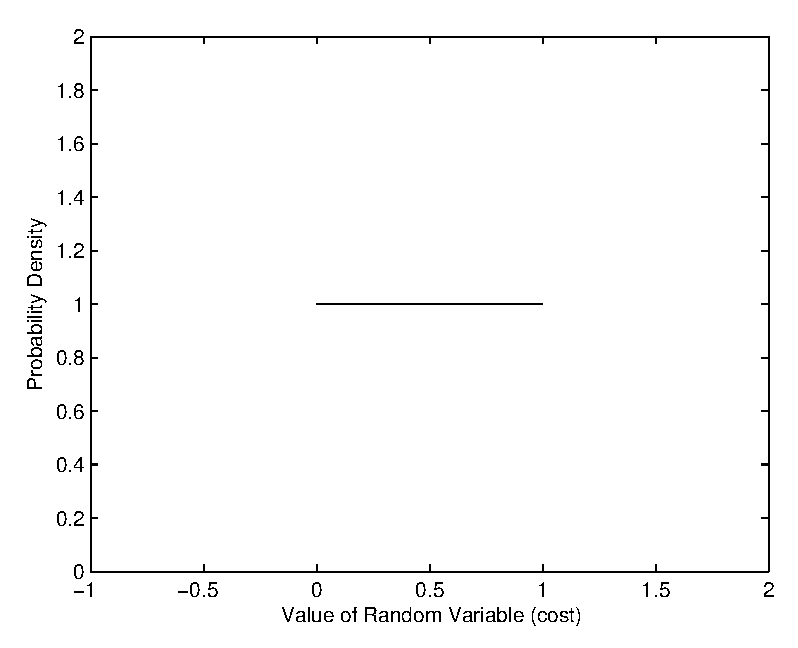
\includegraphics[width = \textwidth]{bayesian_uniform_density_scheme.eps} 
    \caption{均匀分布的概率密度函数} 
    \label{fig:chap_bayesian:uniform_density_scheme} 
  \end{minipage}% 
  \begin{minipage}[t]{0.5\linewidth} 
    \centering 
    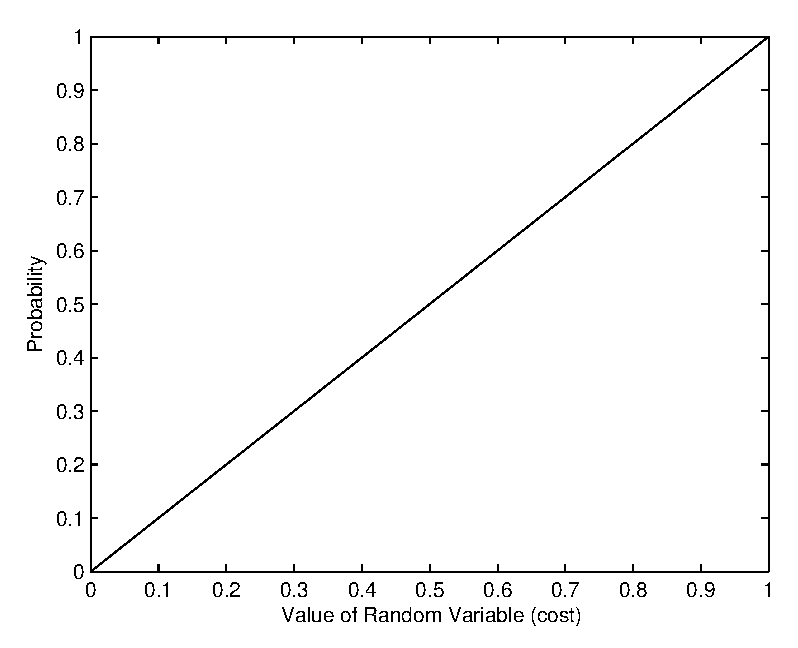
\includegraphics[width=\textwidth]{bayesian_uniform_cdf_scheme.eps} 
    \caption{均匀分布的累积概率函数} 
    \label{fig:chap_bayesian:uniform_cdf_schem} 
  \end{minipage} 
\end{figure}
则达到临界成本~$c^*$~来说,选择“同意”的概率为
\begin{align} 
    P(c^*) &= \text{Prob} \Bigl\{ 0 < c_i < c^*\Bigr\} \notag\\ 
    &= \frac{c^*}{C_{\max}-C_{\min}} \notag\\
    &= c^* 
    \label{eqn_probability_of_contribution} 
\end{align}
把\eqref{eqn_probability_of_contribution}代入\eqref{eqn:chap_bayesian:equilibrium_cost_equation}则有
\begin{align*} 
    c^* &= b - \tau + (1-c^*)^{N-1}\tau
\end{align*}

我们通过做图的方式来直观地讨论在均匀分布的情况下,各个参数对于临界成本和参与者决策的影响,
如\figref{fig:bayesian_user_numb_vs_contr_prob}和\figref{fig:bayesian_puni_para_vs_cont_prob}所示。
图中所涉及的奖励~$b$~,惩罚~$\tau$~都是归一化后,且为了简单起见,~$b = 1$~。
%%%%%%%%%%%%%%%%%%%%%%%%%%%%%%%%%%%%%%%%%%%%%%%%%%%%%%%%%%%%%%%%%%%%%
\begin{figure}[tb]
\begin{centering}
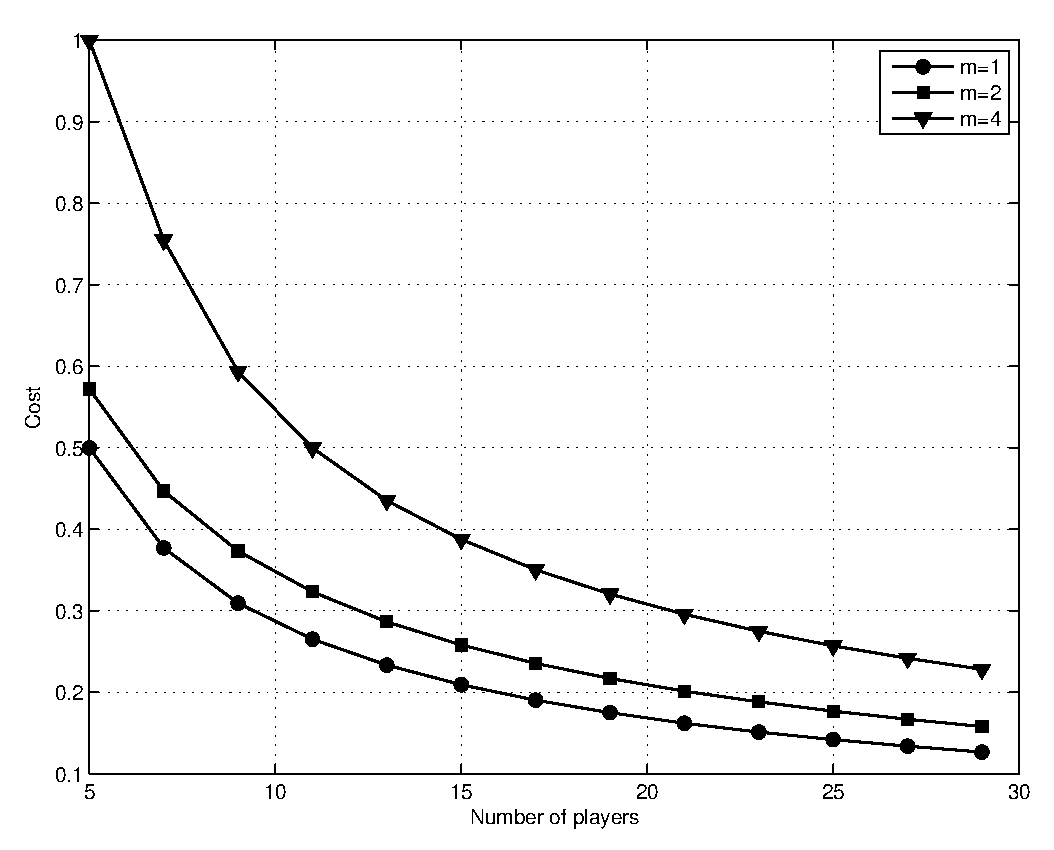
\includegraphics[scale=0.7]{bayesian_uniform_user_number_vs_contribute_probability.eps}
\caption{参与者数目与临界成本的关系,$\tau=0.5, b=1$}
\label{fig:bayesian_user_numb_vs_contr_prob}
\end{centering}
\end{figure}
%%%%%%%%%%%%%%%%%%%%%%%%%%%%%%%%%%%%%%%%%%%%%%%%%%%%%%%%%%%%%%%%%%%%
%%%%%%%%%%%%%%%%%%%%%%%%%%%%%%%%%%%%%%%%%%%%%%%%%%%%%%%%%%%%%%%%%%%%%
\begin{figure}[tb]
\begin{centering}
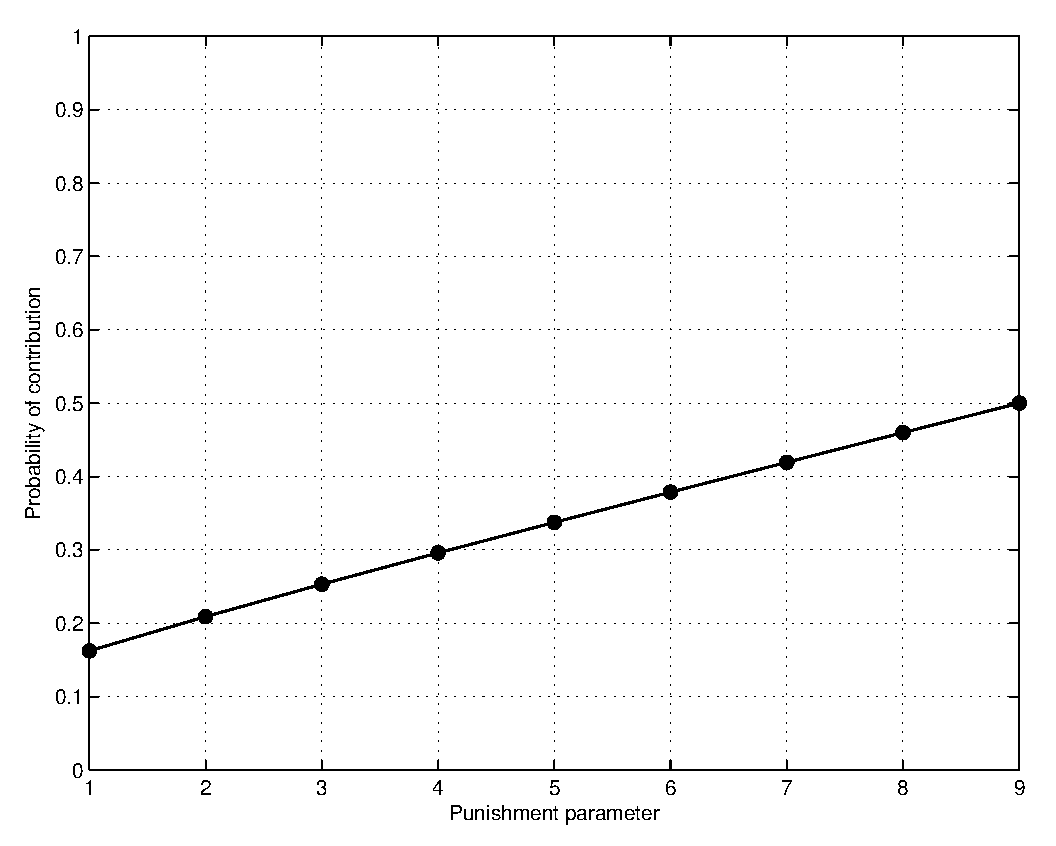
\includegraphics[scale=0.7]{bayesian_uniform_punish_parameter_vs_contribute_probability.eps}
\caption{惩罚系数与临界成本之间的关系,$N=4, b=1$}
\label{fig:bayesian_puni_para_vs_cont_prob}
\end{centering}
\end{figure}
%%%%%%%%%%%%%%%%%%%%%%%%%%%%%%%%%%%%%%%%%%%%%%%%%%%%%%%%%%%%%%%%%%%%
从\figref{fig:bayesian_user_numb_vs_contr_prob}可以看到,
当博弈的参与者总数增多时,临界成本~$c^*$~会减小。
前面我们提到,当博弈参与者的成本~$c_i$~在区间~$ [C_{\min}, c_i^*] $~,参与者的决策就是“同意”。
因而,最终博弈均衡中选择“同意”的概率~$P(c_i^*)$~也会随之降低。
这意味着,当系统中参与者较少时,参与者容易做出接受资源调整的决策。
而当系统参与者较多时,即使参与者的收益比成本高,参与者也可能会做也拒绝的决定。
这说明,当用户总数目多的情况下,自私的用户都希望他人来做出资源占用的调整,而自身却“拒绝”调整。
并且,从中还可以看到临界成本在参与者数目逐渐增多时,存在极限~$b-\tau$~。
另外,
从\figref{fig:bayesian_puni_para_vs_cont_prob}可以看到,当惩罚系数的值增大时,并不会让参与者决策均衡中“同意”的机率增大。这一点与我们的直觉是不同的。
因此在系统中设置一个能够自适应网络状态的奖励参数和惩罚参数的组合是十分必要的。

\subsection{正态分布的情况}
对于参与者的成本类型,第二种我们假设的概率分布是正态分布。
也是一个在数学、物理及工程等领域都非常重要的概率分布。
对于参与者成本随机变量~$c$~服从一个位置参数为~$\mu$~,尺度参数为~$\sigma$~的概率分布,
通常可以记为:
\begin{align*}
    c \sim N(\mu, \sigma^2)
    %\label{eqn:normal_distribution}
\end{align*}
服从正态分布的随机变量的概率密度函数~$f(x)$~由\eqref{eqn:chap_bayesian:normoal_density}和\eqref{eqn:chap_bayesian:normoal_cdf}给出,
且其概率密度函数和概率分布函数如\figref{fig:chap_bayesian:normal_density_scheme}和\figref{fig:chap_bayesian:normal_cdf_schem}所示。
其中,与均匀分布类似的,为了将成本随机变量控制在区间~$[0,1]$~,我们假设成本概率分布的均值为~$\mu = 0.5$~,方差~$\delta = 0.1$~。
\begin{align}
    f(x) = \frac{1}{\sigma \sqrt{2\pi} } e^{ \frac{-(c-\mu)^2}{2\sigma^2}}
    \label{eqn:chap_bayesian:normoal_density}
\end{align}
\begin{align}
    F(x) = \frac{1}{\sigma \sqrt{2\pi} } \int^x_{-\infty}e^{ \frac{-(c-\mu)^2}{2\sigma^2}}
    \label{eqn:chap_bayesian:normoal_cdf}
\end{align}
%%%%%%%%%%%%%%%%%%%%%%%%%%%%%%%%%%%%%%%%%%%%%%%%%%%%%%%%%%%%%%%%%%%%%
\begin{figure}[tb] 
  \begin{minipage}[t]{0.5\linewidth} 
    \centering 
    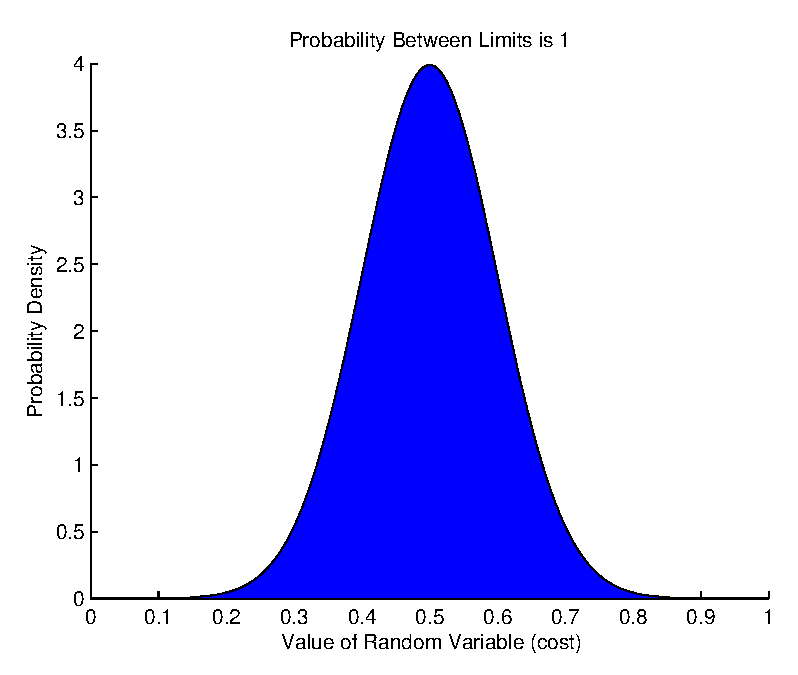
\includegraphics[width = \textwidth]{bayesian_normal_density_scheme.eps} 
    \caption{正态分布的概率密度函数} 
    \label{fig:chap_bayesian:normal_density_scheme} 
  \end{minipage}% 
  \begin{minipage}[t]{0.5\linewidth} 
    \centering 
    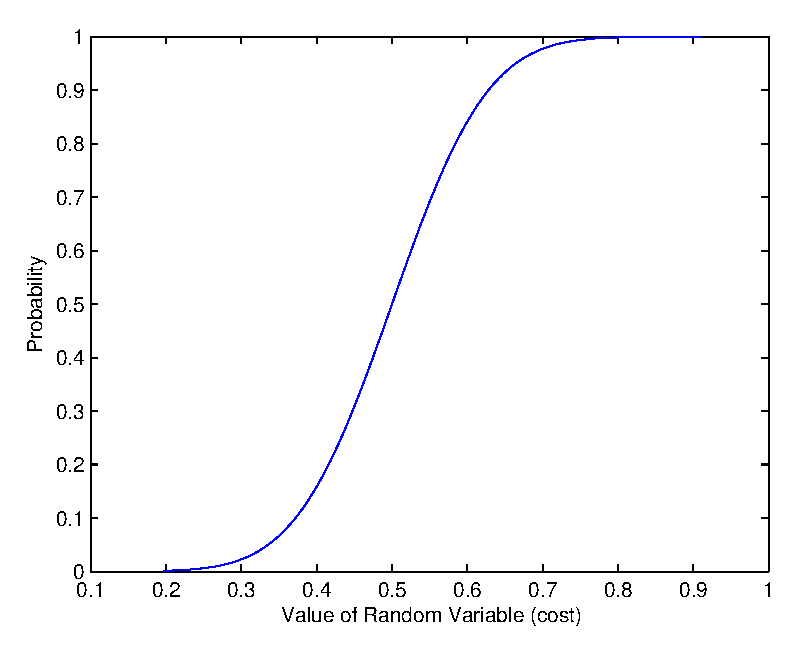
\includegraphics[width=\textwidth]{bayesian_normal_cdf_scheme.eps} 
    \caption{正态分布的累积概率函数} 
    \label{fig:chap_bayesian:normal_cdf_schem} 
  \end{minipage} 
\end{figure}
类似的,如果将\eqref{eqn:chap_bayesian:normoal_cdf}代入\eqref{eqn:chap_bayesian:equilibrium_cost_equation},
则有,
\begin{align} 
    c^* &= b - \tau + \left[ 1-\frac{1}{\sigma \sqrt{2\pi} } \int^x_{-\infty}e^{ \frac{-(c^*-\mu)^2}{2\sigma^2}} \right] ^{N-1}\tau
    \label{eqn:chap_bayesian:cost_normal_distribution_equation}
\end{align}
由于正态分布函数概率密度函数不能显式积分,所以我们只能通过数值求解的方式,将收益参数、惩罚参数、参与者数目与均衡概率关系画出来。
如\figref{fig:bayesian_normal_user_numb_vs_contr_prob}和\figref{fig:bayesian_normal_puni_para_vs_cont_prob}所示。
%%%%%%%%%%%%%%%%%%%%%%%%%%%%%%%%%%%%%%%%%%%%%%%%%%%%%%%%%%%%%%%%%%%%%
\begin{figure}[tb]
\begin{centering}
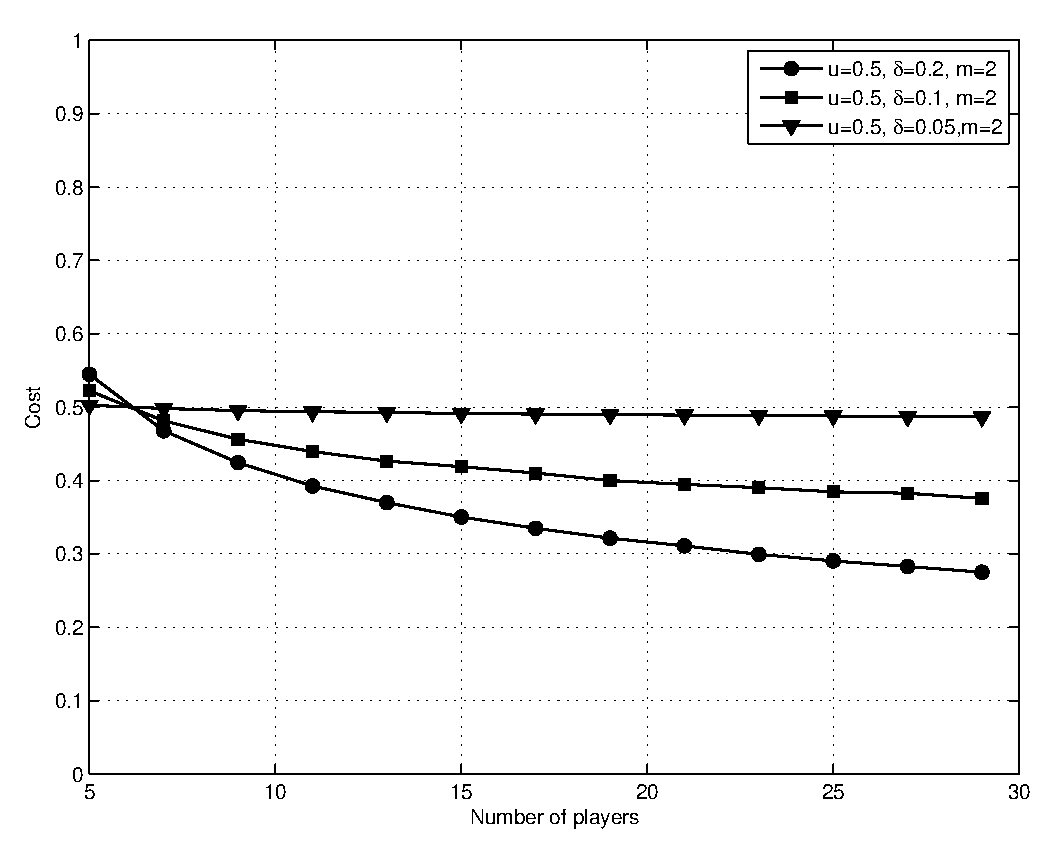
\includegraphics[scale=0.6]{bayesian_normal_user_number_vs_contribute_probability.eps}
\caption{参与者数目与临界成本的关系,$\tau=0.5, b=1$}
\label{fig:bayesian_normal_user_numb_vs_contr_prob}
\end{centering}
\end{figure}
%%%%%%%%%%%%%%%%%%%%%%%%%%%%%%%%%%%%%%%%%%%%%%%%%%%%%%%%%%%%%%%%%%%%
%%%%%%%%%%%%%%%%%%%%%%%%%%%%%%%%%%%%%%%%%%%%%%%%%%%%%%%%%%%%%%%%%%%%%
\begin{figure}[!tb]
\begin{centering}
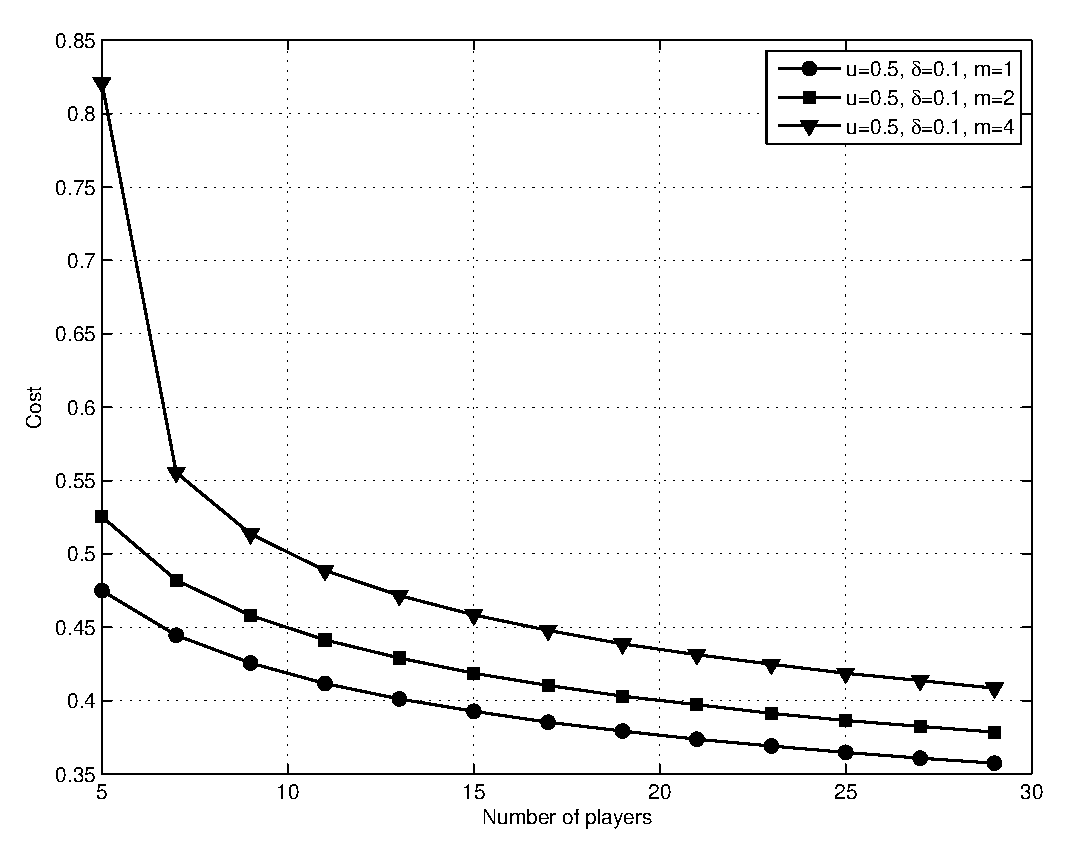
\includegraphics[scale=0.6]{bayesian_normal_punish_parameter_vs_contribute_probability.eps}
\caption{惩罚系数与临界成本之间的关系,$N=4, b=1$}
\label{fig:bayesian_normal_puni_para_vs_cont_prob}
\end{centering}
\end{figure}

与均匀分布的情况十分相似,
当博弈的参与者总数增多时,临界成本~$c^*$~会减小, 如\figref{fig:bayesian_normal_user_numb_vs_contr_prob}如示。
同样,最终混合策略的均衡中选择“同意”的概率~$P(c_i^*)$~也会随之降低。
同理,当系统中参与者较少时,参与者容易做出接受资源调整的决策。
我们还绘制了正态分布的尺度参数~$\delta$~对临界成本的影响。
当尺度参数的值较小时,意味着博弈参与者的类型分布集中比较集中。
在这情况下,临界成本相比较也小。这说明当用户分类少的情况下,博弈参与者选择“同意”的概率也较低。
同样,临界成本在参与者数目逐渐增多时,也会逐渐收敛到~$b-\tau$~。
\figref{fig:bayesian_normal_puni_para_vs_cont_prob}也表明,
当惩罚系数的值增大时,参与者决策均衡中“同意”的机率会减小。这一点与均匀分布一样。
用户类型较多情况比用户类型较单一的情况,“同意”的概率下降更快。
所以,下面我们提出一个能够自适应网络状态的奖励参数和惩罚参数的算法用来调节用户的行为的组合是十分必要的。

\section{基于博弈的资源比例分配算法}
根据上面分析,我们让用户来自身决定如何调整自身目前资源占用的情况。
而控制单元,每隔一个时间间隔,收集各个参与者的业务类型值,汇总以后,进行参数估计,计算均值与方差,并广播给当前服务区的用户。
譬如,对于参与者而言,它根据当前业务分布决策后,应将把自身的业务类型报告给资源分配单元。
%,而不是具体的带宽值或是信道个数。,就可以得到所需的资源。
资源分配单元只是计算一下此用户类型值大小占全部用户类型值之和的比例,然后再按这个比例协调相应的资源给这个用户。
也就是说,这个资源的比例为:
\begin{equation}
    c_i = \frac{c_i}{\sum_{j=1}^N c_j}
    \label{eqn:chap_bayesian:resource_ratio}
\end{equation}
此分配算法的具体流程如下:

\section{仿真实验与结果}

\section{小结}
本章针对网络中业务逐渐增多的趋势,提出通过概率连续随机变量来描述用户的业务类型。
与传统的离散分类不同,新的方法可以更加细致地刻化用户业务特征。
并且根据网络的实际情况,我们提出在不完备信息的情况下通过构造Bayesian博弈模型的方法来寻求使得所有用户满意的资源分配混合策略。
通过理论的分析与仿真实验证明,所提出的业务描述方法及博弈算法,可以有效地解决在多用户竞争下的资源分配问题。


